\documentclass{article}
\usepackage{url}
\usepackage{graphicx}
\usepackage{float}
\usepackage{biblatex}
\addbibresource{ref.bib}
\graphicspath{{./images}}
\title{Analysis of Sample3.dll \\Practical Assignment 3\\Malware Reverse Engineering \\
CAP6137}
\author{Michael Ivanov \\
ivanovmichael@ufl.edu}
\date{March 14, 2022}
\hfuzz=30pt

\begin{document}
    \maketitle
    \pagebreak
    \section{Executive Summary}
    \pagebreak
    \section{Static Analysis}
    \subsection{MD5 Hashes}
    \begin{itemize}
        \item sample3.dll: 3AC8BFD8DA5D3C4789D1F5D26E0E082B
        \item unknown resource: 30245F444D61C3C8780A7058381E140A
    \end{itemize}
    \subsection{Compilation date}
    \begin{itemize}
        \item Sample3.dll: Fri Mar 04, 07:51:31 2022
    \end{itemize}
    \subsection{Suspicious Imports}
    One thing to note is that according to Pestudio, 44 imports are referenced by ordinal.
    \begin{itemize}
        \item \textbf{RegCreateKeyA, RegDeleteValueA, RegSetValueA, RegDeleteKeyA}: these are indicators the malware will probably be modifying the registry.
        \item \textbf{FindFirstFileA, UnlockFile, LockFile, DeleteFileA, MoveFileA}: various file operations
        \item \textbf{GetAtomNameA, GlobalGetAtomNameA, GlobalFindAtomA, GlobalAddAtomA, GlobalDeleteAtom}: Possible dynamic data exchange, which allows for different processes to communicate with each other. \cite{atom}
        \item \textbf{RegisterClipboardFormatA,} \textbf{OleSetClipboardFormatA,} \textbf{OleFlushClipboard}: various clipboard operations.
    \end{itemize}
    \subsection{Suspicious strings}
    The following strings start with \url{f:\dd\vctools\vc7libs\ship\atlmfc\src\mfc\}
    \begin{itemize}
        \item \url{dockcont.cpp}, \url{filecore.cpp}, \url{winctrl2.cpp}, \url{appcore.cpp}, \url{aucdata.cpp}, \url{olefact.cpp}, \url{olestrm.cpp}
    \end{itemize}
    The following strings start with \url{f:\dd\vctools\vc7libs\ship\atlmfc\include\}
    \begin{itemize}
        \item \url{afxwin1.inl}, \url{afxwin2.inl}
    \end{itemize}
    Potential format strings for shell commands:
    \begin{itemize}
        \item \url{%s\shell\open\%s}
        \item \url{%s\shell\print\%s}
        \item \url{%s\shell\printto\%s}
        \item \url{%s\ShellNew}
    \end{itemize}
    A format string for a dll file:
    \begin{itemize}
        \item \url{%s%s.dll}
    \end{itemize}
    \subsection{Program Sections}
    In the resource section (\url{.rsrc}) there is an unknown file. I've provided the hash above. The file seems to be encoded.
    \subsection{Exports}
    \begin{figure}[H]
        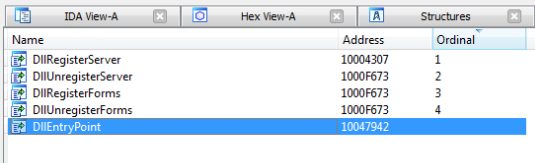
\includegraphics[width=\textwidth]{dllentrypoints.png}
        \caption{List of all exports for sample3.dll using \textit{Ida Pro}}
    \end{figure}
    Using Ghidra I was able to determine that ordinal 1 entry point \textit{DLLRegisterServer} was the most interesting. The rest of the entry points were duplicates of each other and did not do anything.
    \begin{figure}[H]
        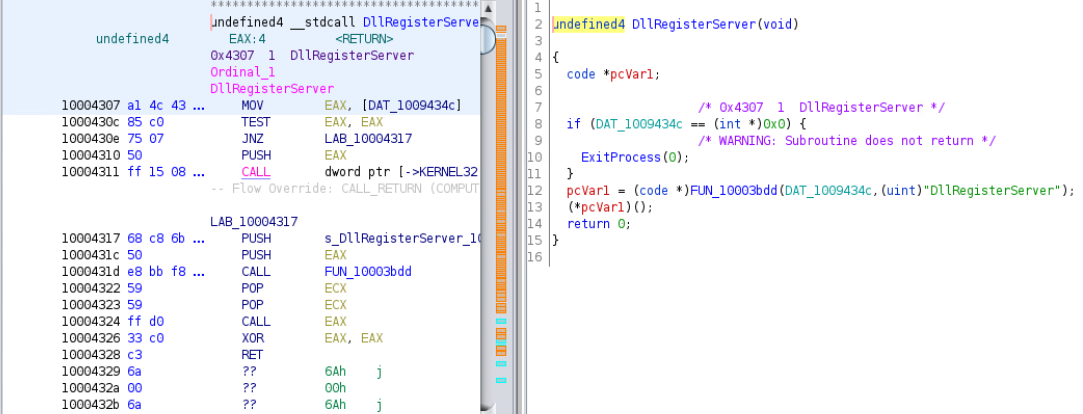
\includegraphics[width=\textwidth]{export1.png}
        \caption{Ordinal 1 entry point \textit{DLLRegisterServer}}
    \end{figure}
    \begin{figure}[H]
        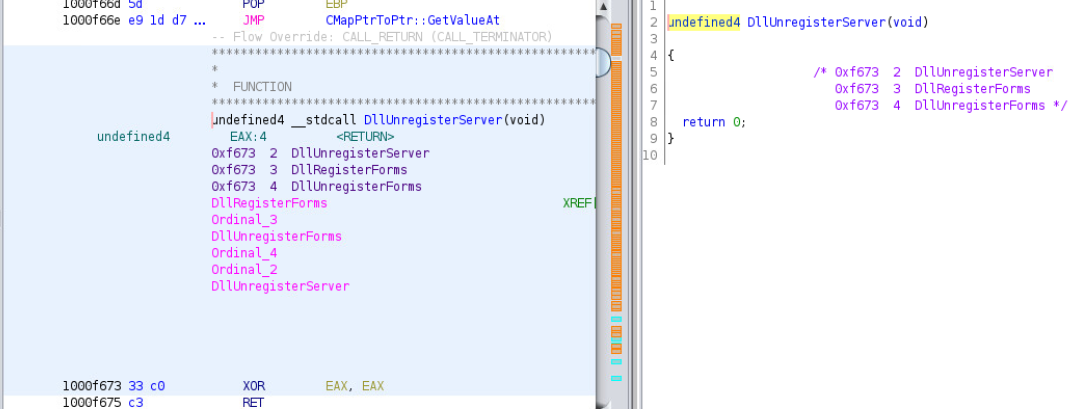
\includegraphics[width=\textwidth]{exports2-4.png}
        \caption{Ordinals 2-4 empty entry points}
    \end{figure}
    \subsection{Anti-disassembly}
    I was not able to find any signs of anti-disassembly.
    \subsection{Anti-debugging}
    \begin{figure}[H]
        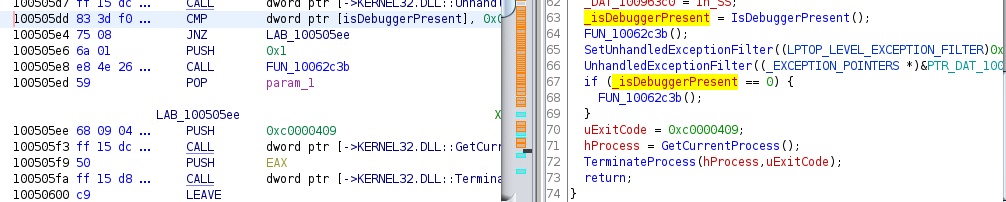
\includegraphics[width=\textwidth]{antidebuging.png}
        \caption{A check in a function at the end of DLLMain for debugging}
    \end{figure}
    \subsection{Obfuscation}
    Below is an indirect call inside the ordinal 1 entry point. The function above returns the address to the call.
    \begin{figure}[H]
        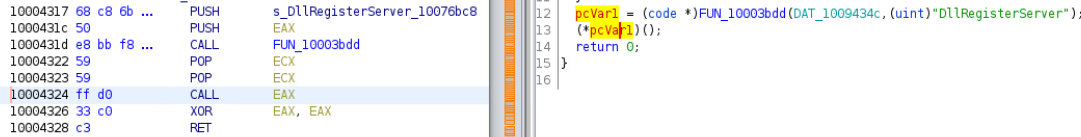
\includegraphics[width=\textwidth]{ord1obf.png}
        \caption{Ordinal 1 entry disassembly of an indirect call}
    \end{figure}
    In the \textit{DLLEntryPoint} there are numerous examples of obfuscation of data. Below is an example found in DLLMain:
    \begin{figure}[H]
        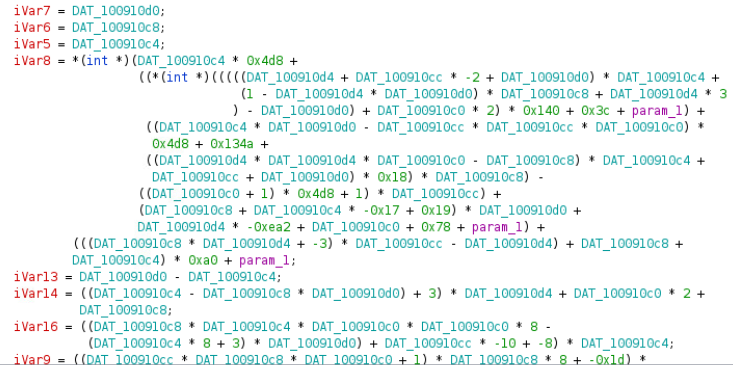
\includegraphics[width=\textwidth]{obfex.png}
        \caption{Example of obfuscation of data}
    \end{figure}
    \pagebreak
    \section{Dynamic Analysis}
    \subsection{Interesting behaviors}
    \subsection{Networking activity}
    The following are network traffic found by running sample3.dll on ordinal 1:
    \begin{itemize}
        \item 51.75.33.122:https
        \item 186.250.45.5:http
        \item 168.119.39.118:https
        \item 85.214.67.203:8080
    \end{itemize}
    \begin{figure}[H]
        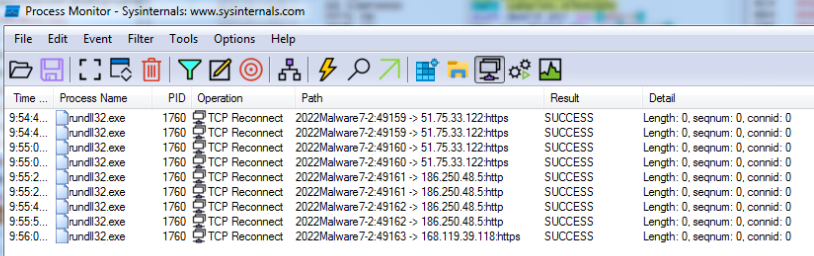
\includegraphics[width=\textwidth]{networkProcmon.png}
        \caption{Example network activity shown by \textit{Procmon}}
    \end{figure}
    \subsection{Registry keys created or modified}
    Registry keys modified:
    \begin{itemize}
        \item \url{HKCU\Software\Microsoft\Windows\CurrentVersion\Internet Settings\Connections\SavedLegacySettings}
        \item \url{HKCU\Software\Microsoft\Windows\CurrentVersion\Internet Settings\ZoneMap\ProxyBypass}
        \item \url{HKCU\Software\Microsoft\Windows\CurrentVersion\Internet Settings\ProxyEnable}
        \item \url{HKCU\Software\Microsoft\Windows\CurrentVersion\Internet Settings\ZoneMap\UNCAsIntranet}
        \item \url{HKCU\Software\Microsoft\Windows\CurrentVersion\Internet Settings\ZoneMap\AutoDetect}
        \item \url{HKCU\Software\Microsoft\Windows\CurrentVersion\Internet Settings\ZoneMap\IntranetName}
        \item \url{HKCU\Software\Microsoft\Windows\CurrentVersion\Internet Settings\Wpad\00-50-56-87-c7-d5\WpadDecisionReason}
        \item \url{HKCU\Software\Microsoft\Windows\CurrentVersion\Internet Settings\Wpad\00-50-56-87-c7-d5\WpadDecisionTime}
        \item \url{HKCU\Software\Microsoft\Windows\CurrentVersion\Internet Settings\Wpad\00-50-56-87-c7-d5\WpadDecision}
        \item \url{HKCU\Software\Microsoft\Windows\CurrentVersion\Internet Settings\Wpad\00-50-56-87-c7-d5\WpadDetectedUrl}
        \item \url{HKCU\Software\Microsoft\Windows\CurrentVersion\Internet Settings\Wpad\{082A014B-1185-406F-8FE4-BB152F2E1081}\WpadDecisionReson}
        \item \url{HKCU\Software\Microsoft\Windows\CurrentVersion\Internet Settings\Wpad\{082A014B-1185-406F-8FE4-BB152F2E1081}\WpadDecisionTime}
        \item \url{HKCU\Software\Microsoft\Windows\CurrentVersion\Internet Settings\Wpad\{082A014B-1185-406F-8FE4-BB152F2E1081}\WpadDecision}
        \item \url{HKCU\Software\Microsoft\Windows\CurrentVersion\Internet Settings\Wpad\{082A014B-1185-406F-8FE4-BB152F2E1081}\WpadNetworkName}
    \end{itemize}
    \begin{figure}[H]
        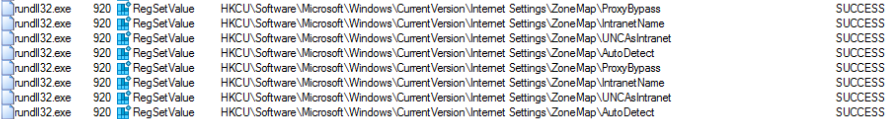
\includegraphics[width=\textwidth]{regkeyset.png}
        \caption{Example registry key activity shown by \textit{Procmon}}
    \end{figure}
    \subsection{Files created or modified}
    \subsection{Processes started}
    \subsection{Persistence}
    \subsection{De-obfuscation}
    \subsection{Anti-debugging}
    The program displayed the message box below due calling \textit{UnhandledExceptionFilter}. This function "\textit{passes unhandled exceptions to the debugger, if the process is being debugged. Otherwise, it optionally displays an Application Error message box and causes the exception handler to be executed}"\Cite{unhandledFilter}.
    \begin{figure}[H]
        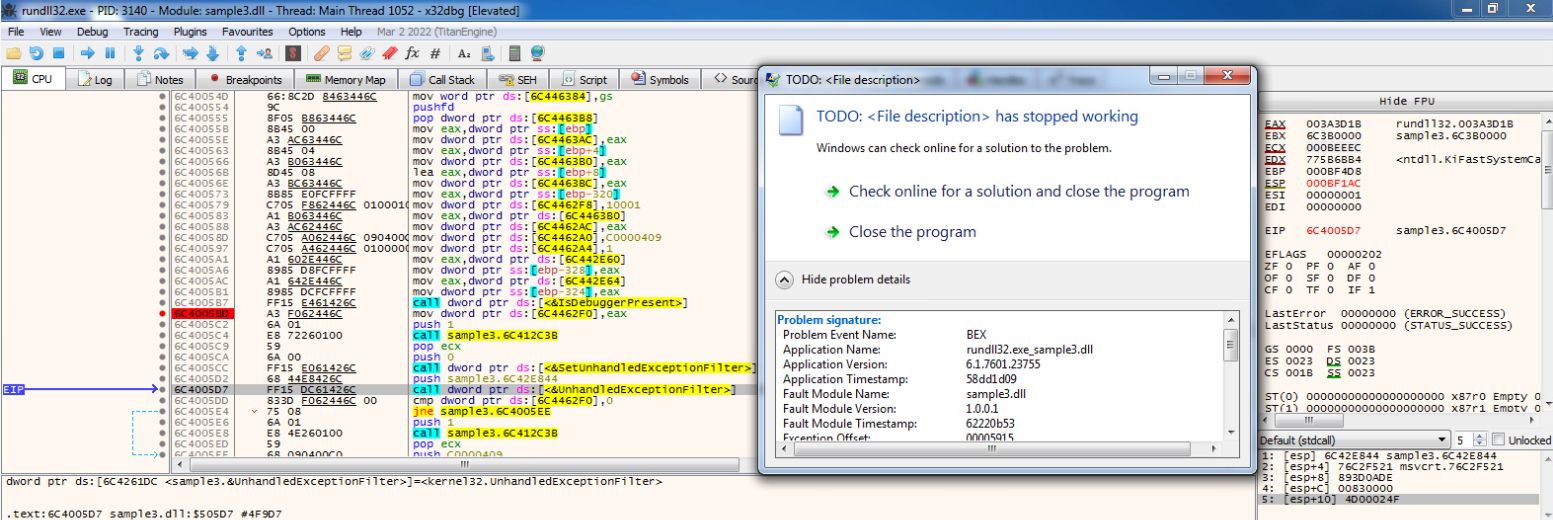
\includegraphics[width=\textwidth]{mesgbox2.png}
        \caption{A message box appearing while debugging}
    \end{figure}
    \pagebreak
    \section{Indicators of Compromise}
    \pagebreak
    \printbibliography
\end{document}